\chapter{Reconhecimento facial}\label{cap:reconhecimento_facial}

Um sistema de reconhecimento facial é uma tecnologia capaz de realizar identificação ou verificação automática de uma pessoa através de uma imagem ou vídeo. 

Segundo \citeonline{jafri2009survey}, essas duas tarefas principais do reconhecimento facial podem ser definidas como:
%
\begin{itemize}
\item \textbf{Verificação} (correspondência um-para-um): dada uma face e uma alegação de identidade, informa se a face realmente pertence ao indivíduo.  

\item \textbf{Identificação} (correspondência de um-para-muitos): compara a imagem de uma face desconhecida com todas as imagens em um banco de dados para determinar sua identidade.
\end{itemize}

Uma terceira tarefa também importante é a de agrupamento (clustering), que consiste em agrupar faces da mesma pessoa mesmo que essa pessoa não esteja cadastrada em um banco. \cite{dhingra2017face, schroff2015facenet}.

São várias as aplicações práticas desses sistemas, como autenticação biométrica, vigilância, interação humano-computador e gerenciamento multimídia. \cite{jain2011handbook}.

O reconhecimento facial possui diversas vantagens sobre outras formas de biometria. Para validação de passaportes, por exemplo, \citeonline{heitmeyer2000biometric} afirma que esse é o método preferido por ser rápido, não intrusivo e poder ser feito à distância sem necessidade de contato.

A tarefa de verificação facial em cenários cooperativos, nos quais as condições de iluminação e pose são controladas, já pode ser considerada um problema bem resolvido. Por outro lado, a identificação um-para-muitos, especialmente em cenários não cooperativos, como busca por pessoas desaparecidas ou procuradas pela polícia, ainda é uma tarefa desafiadora.
A performance do reconhecimento é grandemente influenciada por variações nas condições de iluminação, ponto de vista, poses, expressão facial, envelhecimento, uso de disfarces e acessórios \cite{li2016kernel, jain2011handbook}.

Dentre os trabalhos pioneiros em reconhecimento facial automatizado, destacam-se a tese de doutorado de Takeo Kanade em \citeyear{kanade1973picture}, os trabalhos sobre representação de faces em dimensionalidade reduzida usando PCA feitos por Kirby e Sirovich em \citeyear{sirovich1987low} e \citeyear{kirby1990application} e os trabalhos sobre Eigenfaces de Turk e Pentland em \citeyear{turk1991eigenfaces}.

Outras técnicas relevantes utilizam discriminantes lineares (Fisherfaces LDA) \cite{belhumeur1997eigenfaces, etemad1996face}, local binary patterns (LBP) \cite{ojala1994performance}, filtros de Gabor \cite{lades1993distortion, wiskott1997face, gonccalves2016robusto} e, mais recentemente, GaussianFace (DGP-LVM) \cite{lu2015surpassing} e redes neurais profundas (DNN) \cite{taigman2014deepface, he2015delving, sun2014deep, sun2014predict, sun2015deeply, zhu2014recover, schroff2015facenet, zhou2015naive, yi2014learning, sun2015deepid3, amos2016openface}.

Redes neurais profundas podem ser consideradas o estado da arte em reconhecimento facial. Com taxas de detecção acima de 99,8\% na LFW, esses métodos já ultrapassam a performance humana nesse teste \cite{learned2016labeled, kumar2009attribute}.

O processo de reconhecimento automático de faces envolve três etapas: detecção de faces, extração de características e identificação ou verificação, como ilustrado na \autoref{fig:etapas_reconhecimento}. Na fase de extração de características, é comum realizar uma normalização para alinhar as faces.

\begin{figure}[htbp]
    \caption{Etapas do reconhecimento facial}
    \label{fig:etapas_reconhecimento}
    \begin{adjustbox}{max width=\textwidth}
    \begin{tikzpicture}[
        font=\scriptsize, node distance=2cm,
        mynode/.style={draw, text width=2.5cm, align=center}
        ]
        \node[align=center] (input) {Imagem/\\Vídeo};
        \node[mynode,right=0.5cm of input] (detec) {Detecção\\Facial};
        \node[mynode,right=of detec] (extra) {Extração de\\Características};
        \node[mynode,right=of extra] (recon) {Reconhecimento\\Facial};
        \node[align=center,right=0.5cm of recon] (ident) {Identificação/\\Verificação};
        
        \draw[->,shorten <=1pt,shorten >=1pt] (input) -- (detec);
        \draw[->,shorten <=1pt,shorten >=1pt] (detec) -- node[fill=white] {Faces}(extra);
        \draw[->,shorten <=1pt,shorten >=1pt] (extra) -- node[fill=white] {Modelo}(recon);
        \draw[->,shorten <=1pt,shorten >=1pt] (recon) -- (ident);
    \end{tikzpicture}
    \end{adjustbox}
\end{figure}

Os algoritmos Eigenfaces, Fisherfaces e Local Binary Patterns Histograms (LBPH) estão implementados na biblioteca OpenCV \cite{opencvreconhecimento}.


\section{Extração de características}\label{sec:extract_caract}

Imagens digitais são representadas por milhares de pixels que são codificados em arrays de alta dimensionalidade. Os métodos de extração de características procuram encontrar as informações mais relevantes das imagens originais e representá-las em um espaço de menor dimensionalidade.

Existem $256^{10000}$ formas diferentes de formar uma imagem em tons de cinza (8 bits) de $100\times100$ pixels, mas apenas uma pequena fração dessas imagens representam faces. Além disso, muitas características são comuns a todas as faces e não são úteis para diferenciá-las.

A redução da dimensionalidade do espaço permite eliminar essas redundâncias e características indesejadas. Ela pode ser realizada se o erro quadrático médio (EQM) ou a soma da variância dos elementos forem mínimas, o que é verdade para imagens de faces por elas compartilharem muitas similaridades.

%%%% TODO: Talvez mover para eigenfaces?
Como explicado por \citeonline{datta2015face}, a ideia principal dos métodos de reconhecimento facial baseados em subespaço é encontrar vetores que melhor representam a distribuição de faces em todo o espaço da imagem. Esses vetores de dimensão reduzida definem o subespaço das faces. Após a linearização, o vetor médio entre todas as imagens de faces é calculado e subtraído de cada vetor correspondente às faces originais. Depois, a matriz de covariância é calculada para extrair um número limitado de autovetores, correspondentes aos maiores autovalores. Esses autovetores, também chamados eigenfaces, representam uma base em um espaço de baixa dimensionalidade. Para testar uma imagem, sua eigenface é calculada e comparada com todas as faces no banco de dados.

Os principais métodos que utilizam subespaços para reconhecimento facial são o PCA e o LDA \cite{wang2004unified}. O PCA seleciona as características que melhor representam a face e o LDA seleciona o subespaço que melhor discrimina classes de faces. Eles também podem ser utilizados em conjunto.


\subsection{Análise de componentes principais (PCA)}\label{sec:pca}

A análise de componentes principais (em inglês, principal component analysis ou PCA) é uma técnica de redução de dimensionalidade inventada em 1901 por \citeonline{pearson1901liii}.
Em \cite{gerbrands1981relationships} foi concluído que PCA é o mesmo que a transformada de Karhunen-Loève (KLT) exceto por uma possível mudança na origem do sistema de coordenadas.
Em \cite{andrews1975two} foi alertado que, apesar de próximos, SVD (decomposição em valores singulares) não é o mesmo que PCA e KLT. 

\begin{figure}[htbp]
    \caption{Análise de Componentes Principais}
    \label{fig:pca}
    \begin{subfigure}[c]{0.45\textwidth}
    \centering
    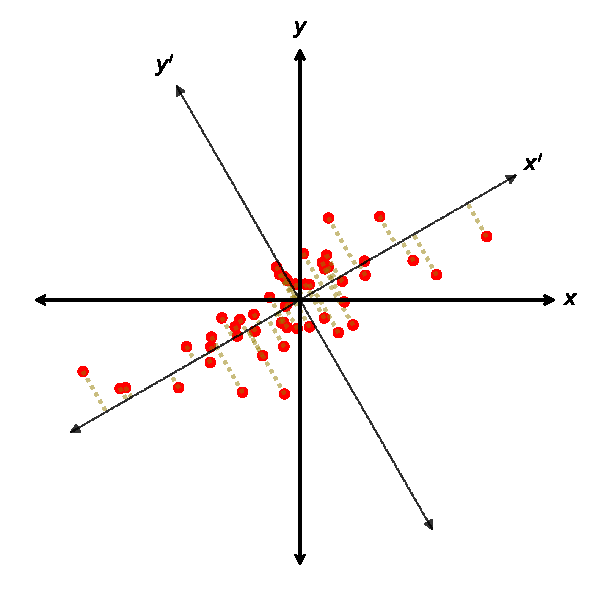
\includegraphics[width=\textwidth]{imagens/pca1.pdf}
    \caption{Distribuição original}
    \end{subfigure}
    \begin{subfigure}[c]{0.45\textwidth}
    \centering
    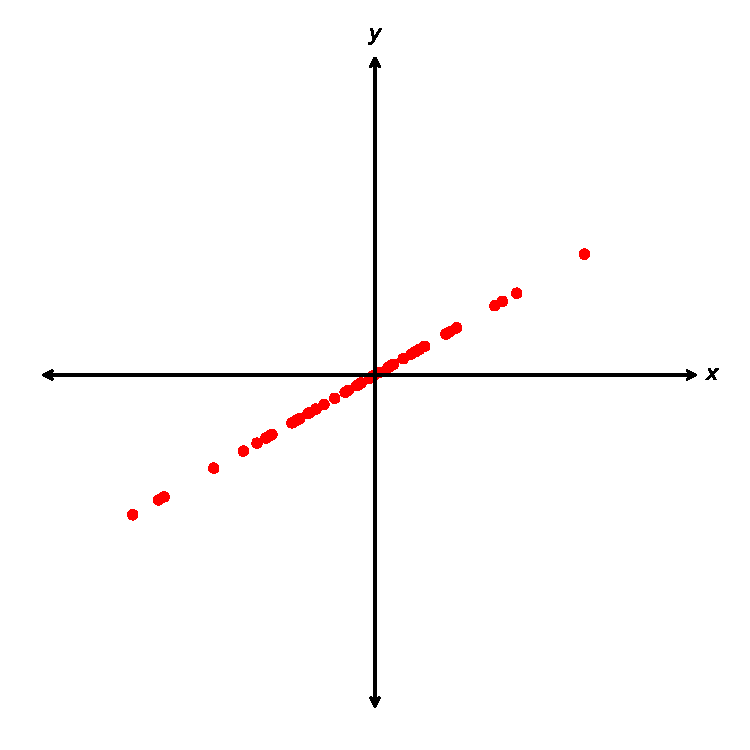
\includegraphics[width=\textwidth]{imagens/pca2.pdf}
    \caption{Apenas o primeiro componente principal}
    \end{subfigure}
\end{figure}

Segundo \cite{jolliffe2002principal}, a ideia central da análise de componentes principais (PCA) é reduzir a dimensionalidade de um conjunto de dados que consiste em um grande número de variáveis, mantendo o máximo possível da variação presente no conjunto de dados. Isto é alcançado através da transformação para um novo conjunto de variáveis, os componentes principais, que não são correlacionados e são ordenados de forma que os primeiros retenham a maior parte da variação presente em todas as variáveis originais.

O conceito do PCA está ilustrado na \autoref{fig:pca}. Os eixos $x$ e $y$ formam a base original e o eixo $x'$ corresponde à direção de maior variância, ou seja, ao primeiro componente principal.

Matematicamente, dados $n$ pontos em $\mathbb{R}^p$, a PCA consiste em escolher uma dimensão $k < p$ e encontrar um espaço afim de dimensão $k$ onde a distância ao quadrado dos pontos às suas projeções ortogonais no espaço são minimizadas.


\subsection{Eigenfaces}\label{sec:eigenfaces}

As eigenfaces são os componentes principais de uma distribuição de faces, ou seja, os autovetores da matriz de covariância de um conjunto de imagens de faces.
Cada face pode ser representada como uma combinação linear de eigenfaces, como mostra a \autoref{fig:eigenfaces_comblinear}. Elas também podem ser aproximadas usando apenas as eigenfaces que possuem os maiores autovalores e que, consequentemente, são responsáveis pela maior variância.

A ideia de usar componentes principais para representar faces humanas foi desenvolvida por \citeonline{sirovich1987low} e usada por \cite{turk1991eigenfaces} para detecção e reconhecimento facial.
Muitos consideram essa técnica de reconhecimento facial baseada em aparência como a primeira a ser utilizada com sucesso na prática.

\begin{figure}[htbp]
    \centering
    \caption{Representação de uma face como combinação linear de eigenfaces}
    \label{fig:eigenfaces_comblinear}
    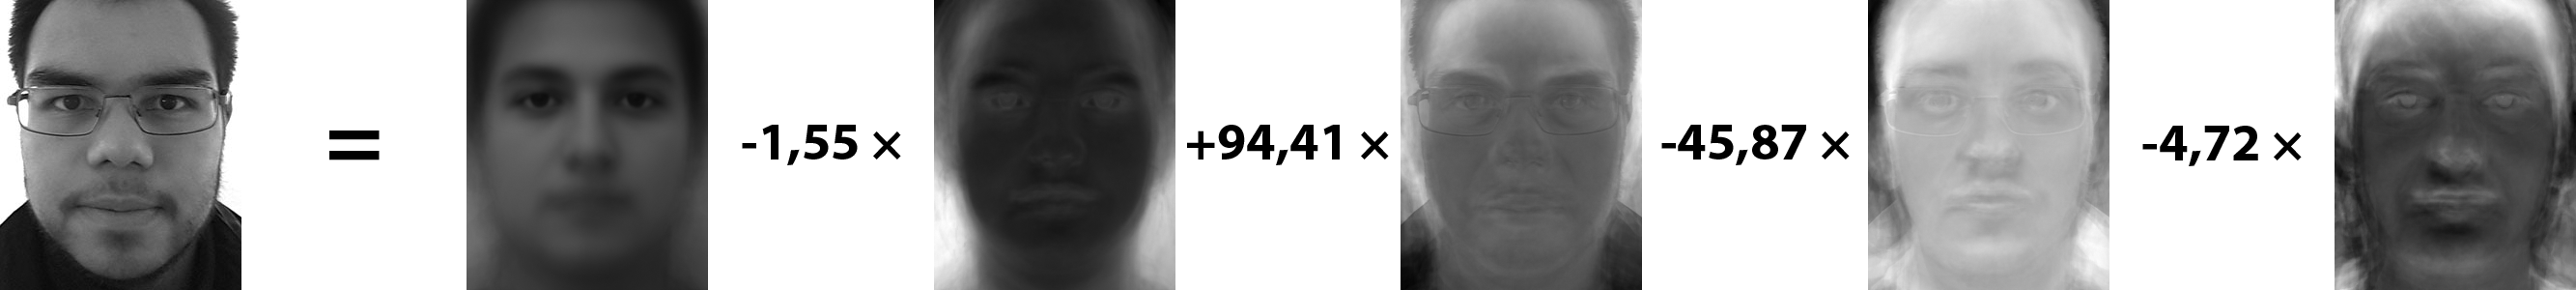
\includegraphics[width=0.95\linewidth]{imagens/eign_lincomb.png}
\end{figure}


\subsubsection{Algoritmo para cálculo das eigenfaces}\label{sec:eigenfaces_algoritmo}

O algoritmo para a obtenção das eigenfaces proposto por \citeonline{turk1991face} pode ser formulado da seguinte forma:

\begin{enumerate}
    \item Obter $M$ imagens $I_1, I_2, I_3 \ldots I_M$ com dimensão $N \times N$.
    As imagens devem estar centralizadas.
    \item Representar cada imagem $I_i$ como um vetor $\Gamma_i$ de dimensão $N^2 \times 1$.
    %
    \begin{equation} \label{eq:eign_gamma}
        \begin{bmatrix}
        a_{11} & a_{12} & \cdots & a_{1N}\\ 
        a_{21} & a_{22} & \cdots & a_{2N}\\ 
        \vdots & \vdots & \ddots & \vdots\\ 
        a_{N1} & a_{N1} & \cdots & a_{NN}
        \end{bmatrix}_{N \times N} \rightarrow \begin{bmatrix}
        a_{11}\\ 
        \vdots\\ 
        a_{1N}\\ 
        \vdots\\ 
        a_{2N}\\
        \vdots\\ 
        a_{NN}
        \end{bmatrix}_{N^2 \times 1}
    \end{equation}
    %
    \item Calcular o vetor $\Psi$ correspondente à face média.
    %
    \begin{equation} \label{eq:eign_media}
        \Psi = \frac{1}{M}\sum_{i=1}^{M}\Gamma_i
    \end{equation}
    %
    \item Subtrair a face média de cada vetor $\Gamma_i$ para obter o conjunto de vetores $\Phi_i$.
    %
    \begin{equation} \label{eq:eign_phi}
        \Phi_i = \Gamma_i - \Psi
    \end{equation}
    %
    \item Encontrar a matriz $C$ de covariância.
    %
    \begin{equation} \label{eq:eign_c}
        C = AA^T \text{, onde } A = \begin{bmatrix}\Phi_1  & \Phi_2 & \ldots  & \Phi_3\end{bmatrix}
    \end{equation}
    %
    $C$ é uma matriz $N^2 \times N^2$ e $A$ é uma matriz $N^2 \times M$.
    \item Calcular os autovetores $u_i$ de $C = AA^T$.
    
    Em vez desse cálculo, que resultaria em $N^2$ autovetores, calcular os autovetores $v_i$ da matriz $A^TA$ de dimensão $M \times M$.
    %
    \begin{equation} \label{eq:eign_autov}
    \begin{alignedat}{2}
                     && A^T Av_i    &= \mu_i v_i\\
    \Rightarrow\quad && AA^T Av_i   &= \mu_i Av_i\\
    \Rightarrow\quad && CAv_i       &= \mu_i Av_i\\
    \Rightarrow\quad && u_i         &= Av_i
    \end{alignedat}
    \end{equation}
    %
    ou seja, $Av_i$ são autovetores de $C = AA^T$. Os $M$ autovalores de $A^TA$ correspondem aos $M$ maiores autovalores de $AA^T$.
    \item Manter apenas os $K$ autovetores, correspondentes aos $K$ maiores autovalores.
\end{enumerate}

Cada face $\Phi_i$ (face menos a média), correspondente a uma das $M$ imagens de treinamento, possui uma representação vetorial $\Omega_i$ na base formada pelos $K$ autovetores escolhidos, ou seja, pode ser representada pela seguinte combinação linear:
%
\begin{equation} \label{eq:eign_lincomb}
    \Gamma_i - \Psi = \Phi_i = \sum_{j=1}^{K}w_ju_j, (w_j = u_{j}^{T}\Phi_i)
\end{equation}
%
Cada peso $w_j$ descreve a contribuição do autovetor $u_j$ na representação da imagem. Eles formam o seguinte vetor $\Omega_i$:
%
\begin{equation} \label{eq:eign_lincomb_vetor}
\Omega_i = \begin{bmatrix}
        w_{1}^{i}\\ 
        w_{2}^{i}\\ 
        \vdots\\ 
        w_{K}^{i}
        \end{bmatrix}, i = 1, 2, \ldots, M
\end{equation}
%

\subsubsection{Reconhecimento usando eigenfaces}\label{sec:eigenfaces_reconhecimento}

O reconhecimento de uma face desconhecida $\Gamma$ centralizada e com as mesmas dimensões das imagens de treinamento é feito através dos seguintes passos:

\begin{enumerate}
    \item Normalização da imagem.
        \begin{equation} \label{eq:eign_rec_norm}
            \Gamma: \Phi = \Gamma - \Psi
        \end{equation}
    \item Projeção no autoespaço.
        \begin{equation} \label{eq:eign_rec_lincomb}
            \hat{\Phi} = \sum_{i=1}^{K}w_iu_i, (w_i = u_{i}^{T}\Phi)
        \end{equation}
    \item Representação de $\Phi$ como $\Omega$:
        \begin{equation} \label{eq:eign_rec_omg}
            \Omega = \begin{bmatrix}
            w_{1}\\ 
            w_{2}\\ 
            \vdots\\ 
            w_{K}
            \end{bmatrix}
        \end{equation}
    \item Cálculo da distância (euclidiana) mínima $e_r = min_l\left \| \Omega - \Omega^l \right \|$.
    \item Se a distância $e_r$ foi menor que um limite $T_r$ escolhido, então $\Gamma$ é reconhecida como a face l do conjunto de treino.
\end{enumerate}


\begin{figure}[htbp]
    \centering
    \caption{Eigenfaces}
    \label{fig:eigenfaces_faces}
    \begin{subfigure}[t]{0.3\textwidth}
    \centering
    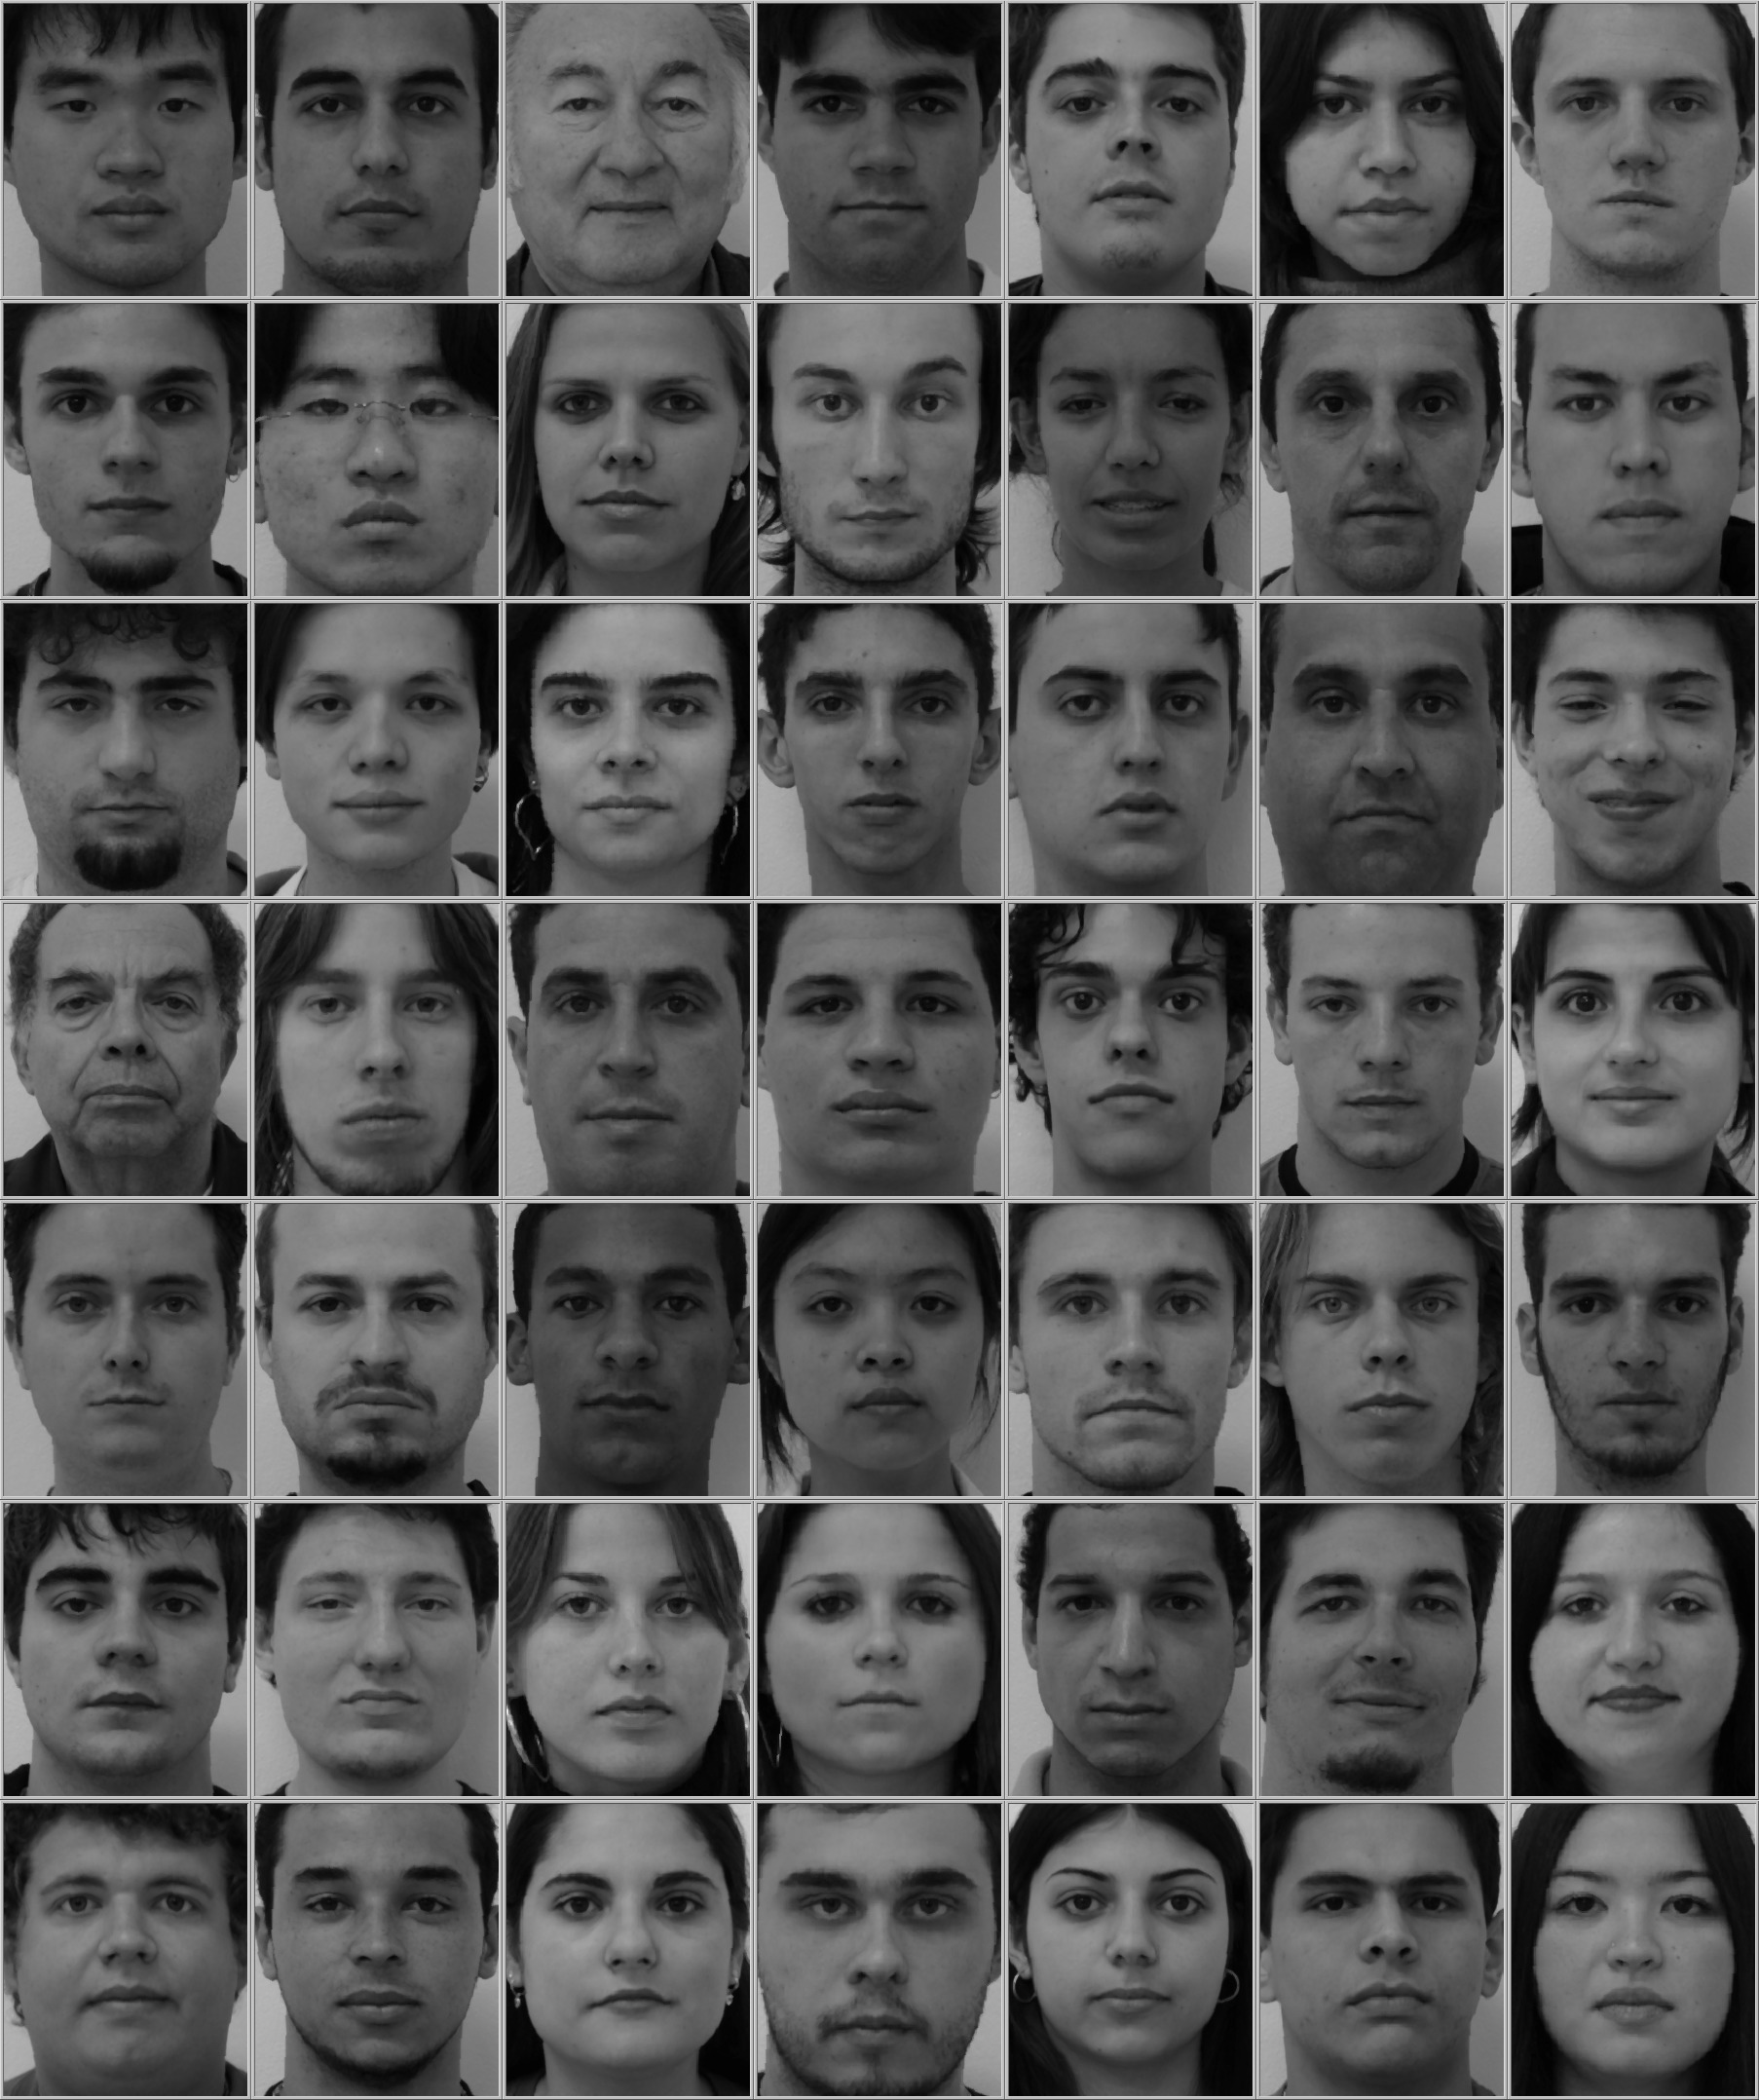
\includegraphics[width=\textwidth]{imagens/faces_fei.jpg}
    \caption{Alguma faces da FEI Face Database}
    \end{subfigure}
    \begin{subfigure}[t]{0.3\textwidth}
    \centering
    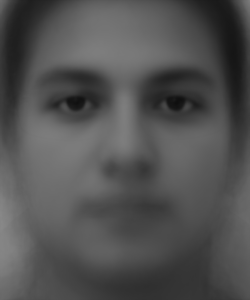
\includegraphics[width=\textwidth]{imagens/face_media.png}
    \caption{Face média}
    \end{subfigure}
    \begin{subfigure}[t]{0.3\textwidth}
    \centering
    
\includegraphics[width=\textwidth]{imagens/eigenfaces.png}
    \caption{Eigenfaces}
    \end{subfigure}
\end{figure}

\subsubsection{Implementação e avaliação do algoritmo}\label{sec:eigenfaces_testes}

O \autoref{cod:eigenfaces_opencv} apresenta como realizar o reconhecimento facial com Eigenfaces utilizando a classe \texttt{EigenFaceRecognizer} da biblioteca OpenCV.

Foram realizados três testes para avaliar o desempenho do algoritmo com diferentes bases de faces. O primeiro utilizou a base da AT\&T, um subconjunto da FERET database foi utilizado para o segundo teste e o terceiro foi feito com algumas imagens selecionadas da Extended Yale Face Database B.

No primeiro teste, foram utilizadas 9 fotos de cada um dos 40 indivíduos para o treino e uma foto de cada para a avaliação.
Das 40 faces de teste, o algoritmo reconheceu 38 faces com sucesso e errou o reconhecimento de duas. A taxa de reconhecimento obtida foi de 95\%, o que sugere que o método das eigenfaces tem bom resultado quando utilizado com imagens frontais de poucas pessoas em ambientes com iluminação controlada. Esse resultado pode ser visto na \autoref{fig:eigenfaces_resultado_att}.

No segundo teste, usando um subconjunto da base de faces FERET composto por 1542 imagens frontais de 865 pessoas para treino e uma foto de avaliação para cada pessoa, o algoritmo obteve 550 acertos e 315 erros, ou seja, uma taxa de apenas 63,6\% de acertos mesmo com pose e iluminação controladas. Isso se deve, provavelmente, pelo grande número de indivíduos e pelo baixo número de imagens de treino por indivíduo.

No terceiro teste, foram utilizadas 49 imagens de cada um dos 38 indivíduos para treinamento e uma foto de cada para testar o reconhecimento. O algoritmo obteve 31 acertos e 7 erros, ou seja, 81,6\% de acertos. Esse resultado está exposto na \autoref{fig:eigenfaces_resultado_yale}.

O reconhecimento facial com eigenfaces é muito vulnerável a mudanças na iluminação e na orientação da face. Em \cite{baggio2012mastering} são dadas algumas sugestões de pré-processamento, ilustradas na \autoref{fig:preprocessamento}, que ajudam a diminuir o impacto desses fatores:
%
\begin{itemize}
    \item \textbf{Transformações geométricas}: redimensionar, rotacionar e transladar a imagem de forma que os olhos fiquem alinhados.
    
    \item \textit{\textbf{Cropping}}: remoção da testa, queixo, orelhas e fundo da imagem.
    
    \item \textbf{Equalização do histograma}: deve ser feito para ambos os lados da face para ajustar o brilho e o contraste em cada lado de forma independente.
    
    \item \textbf{Suavização usando filtros bilaterais}: esse processo reduz o ruído da imagem.
    
    \item \textbf{Máscara elíptica}: máscara que contorna a face a fim de remover o cabelo e o fundo da imagem.
\end{itemize}

\begin{figure}[ht]
    \centering
    \caption[Pré-processamentos para melhorar reconhecimento]{Pré-processamentos sugeridos por \citeonline{baggio2012mastering} para melhorar a performance dos algoritmos de reconhecimento facial}
    \label{fig:preprocessamento}
    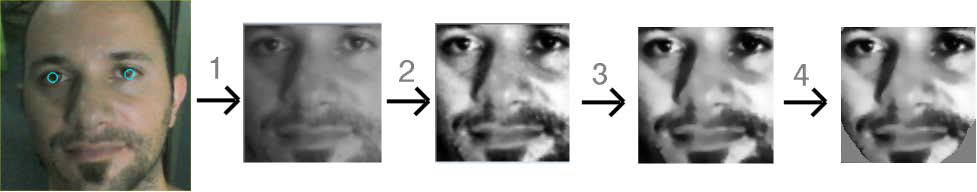
\includegraphics[width=0.95\linewidth]{imagens/preprocessamento.png}
\end{figure}

\begin{figure}[htbp]
    \centering
    \caption[Teste do algoritmo Eigenfaces - AT\&T]{Teste do reconhecimento usando Eigenfaces com a base de faces da AT\&T. Em verde as detecções corretas, em vermelho as erradas}
    \label{fig:eigenfaces_resultado_att}
    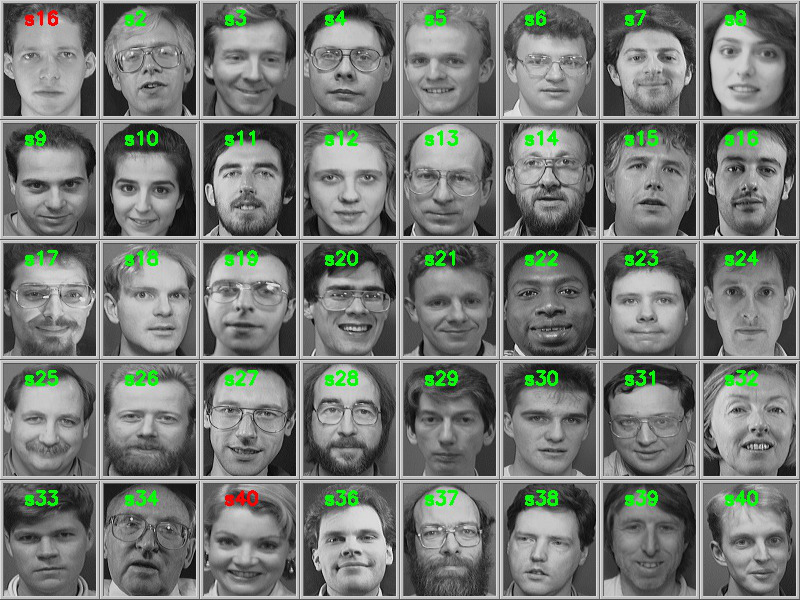
\includegraphics[width=0.8\linewidth]{imagens/eigenfaces_resultado_att.jpg}
    \vspace{\floatsep}
    \caption[Teste do algoritmo Eigenfaces - FERET]{Teste do reconhecimento usando Eigenfaces com a base de faces FERET. Em verde as detecções corretas, em vermelho as erradas}
    \label{fig:eigenfaces_resultado_feret}
    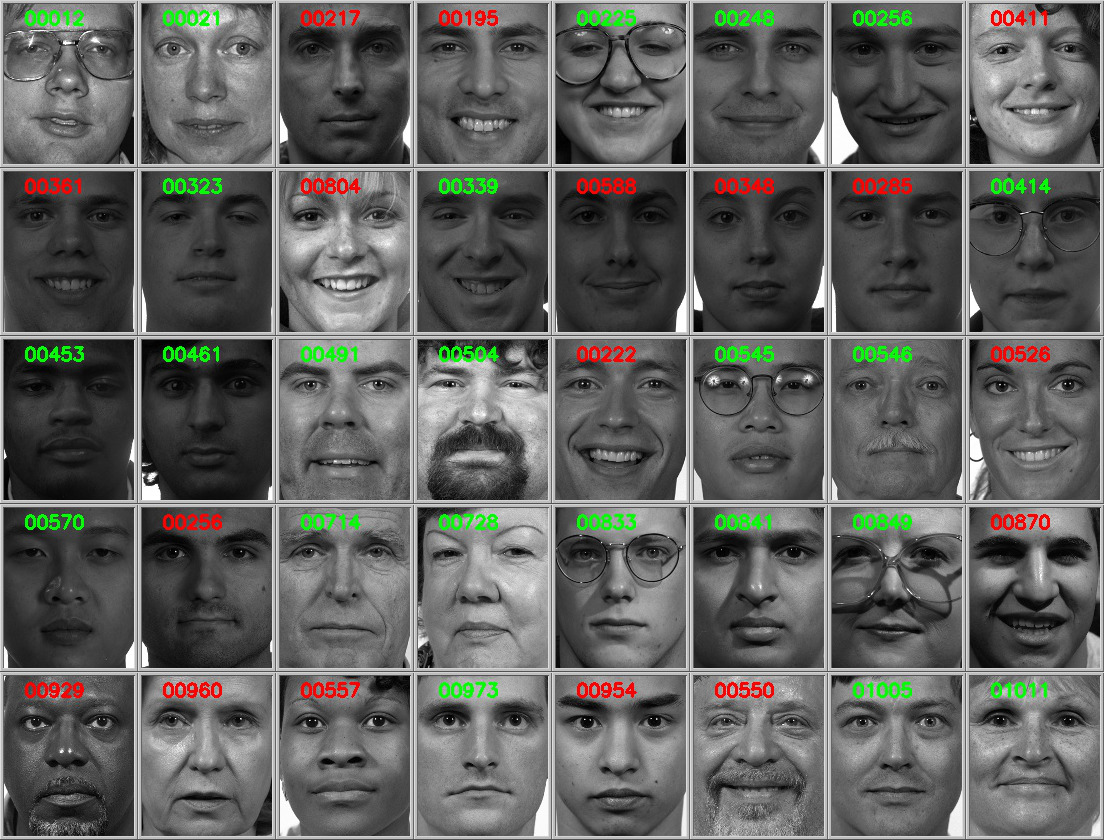
\includegraphics[width=0.8\linewidth]{imagens/eigenfaces_resultado_feret.jpg}
\end{figure}

\begin{figure}[htbp]
    \centering
    \caption[Teste do algoritmo Eigenfaces - Yale]{Teste do reconhecimento usando Eigenfaces com o Extended Yale Face Database B. Em verde as detecções corretas, em vermelho as erradas}
    \label{fig:eigenfaces_resultado_yale}
    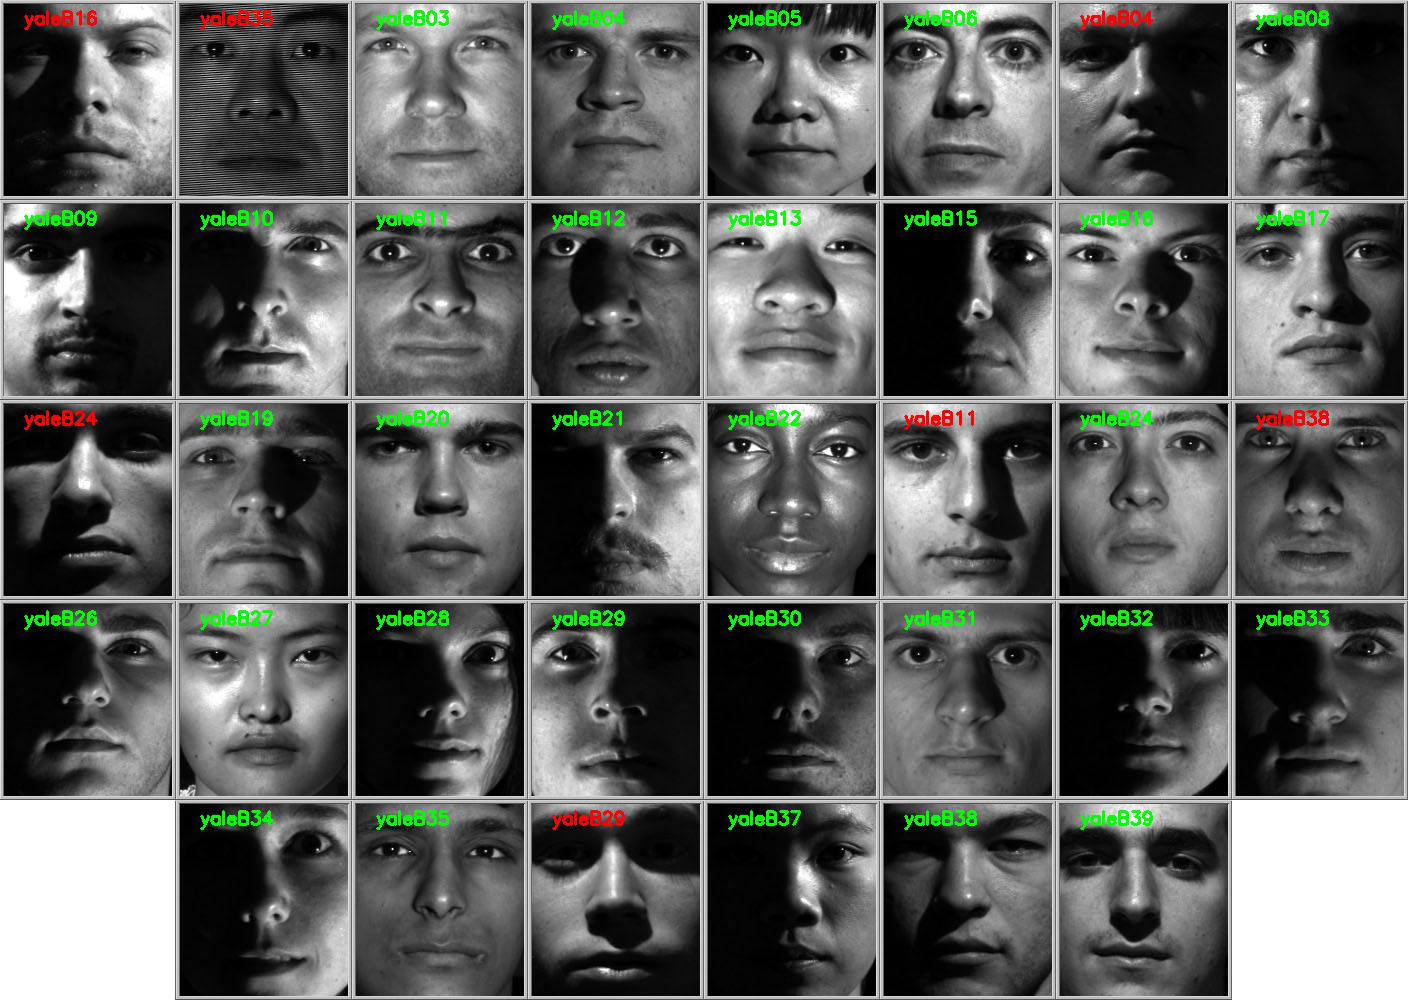
\includegraphics[width=0.95\linewidth]{imagens/eigenfaces_resultado_yale.jpg}
\end{figure}


\Needspace{5\baselineskip}
\subsubsection{Comparação com outros métodos}\label{sec:eigenfaces_comparacao}

Além do Eigenfaces, os métodos Fisherfaces e Local Binary Patterns Histograms também estão implementados na biblioteca OpenCV. Para fins de comparação, os testes realizados com o Eigenfaces também foram realizados com esses dois métodos. Os resultados podem ser vistos na \autoref{tab:compara_reconhecimento} \footnotemark.

\begin{table}[htpb]
\centering
\caption{Bancos de faces utilizados para testes}
\label{tab:bancos_faces}
\begin{tabular}{|l|l|l|}
\hline
\textbf{Banco de faces} & \textbf{Indivíduos} & \textbf{Fotos de treino} \\\hline
\textbf{AT\&T}          & 40                  & 360                      \\\hline
\textbf{FERET}          & 865                 & 1542                     \\\hline
\textbf{Extended Yale}  & 38                  & 1862                     \\\hline
\end{tabular}
\end{table}

\begin{table}[htbp]
\centering
\caption{Comparação dos algoritmos de reconhecimento facial}
\label{tab:compara_reconhecimento}
\begin{tabular}{|c|l|l|l|l|}
\hline
\textbf{Método}                       & \textbf{Banco de faces} & \textbf{Acertos} & \textbf{Erros} & \textbf{Taxa de acertos} \\\hline
\multirow{3}{*}{\textbf{Eigenfaces}}  & AT\&T                   & 38               & 2              & 95,0\%                   \\
                                      & FERET                   & 550              & 315            & 63,4\%                   \\
                                      & Extended Yale           & 31               & 7              & 81,6\%                   \\\hline
\multirow{3}{*}{\textbf{Fisherfaces}} & AT\&T                   & 39               & 1              & 97,5\%                   \\
                                      & FERET\footnotemark[\value{footnote}] & -   & -              & -                        \\
                                      & Extended Yale           & 38               & 0              & 100\%                    \\\hline
\multirow{3}{*}{\textbf{LBPH}}        & AT\&T                   & 40               & 40             & 100\%                    \\
                                      & FERET                   & 786              & 81             & 90,7\%                   \\
                                      & Extended Yale           & 36               & 2              & 94,7\%                   \\\hline
\end{tabular}
\end{table}

\footnotetext{Devido à pouca quantidade de imagens por indivíduo, o teste com a FERET não pode ser realizado com o Fisherfaces.}

Pelos resultados obtidos nos testes realizados neste trabalho e em outros artigos, pode-se concluir que o método de reconhecimento utilizando eigenfaces é bastante rudimentar quando comparado a métodos mais recentes. Seu estudo é importante por ter sido um pioneiro na área de reconhecimento e servido de base para outros algoritmos, porém seu desempenho deixa a desejar, especialmente em ambientes pouco controlados.